\documentclass[oneside]{book}
\usepackage[margin=2cm]{geometry}
\usepackage{amsmath}
\usepackage{amssymb}	
\usepackage{graphicx}
\usepackage{fancyvrb}
\usepackage{color}
\usepackage{xcolor}
\usepackage{float}
\usepackage{listings}
\usepackage{minted}
\usepackage{tabu}
\usepackage{amssymb}
\usepackage{graphicx}
\usepackage{titlesec}
\usepackage[titletoc,toc,page,title,header]{appendix}
\graphicspath{ {.} }

\let\oldemptyset\emptyset
\let\emptyset\varnothing
\newcommand{\HRule}{\rule{\linewidth}{0.5mm}}
\setlength{\parindent}{0in}
\setlength{\parskip}{12pt}

\makeatletter
\renewcommand\chapter{\thispagestyle{plain}%
\global\@topnum\z@
\@afterindentfalse
\secdef\@chapter\@schapter}
\makeatother 

% Solarized colour scheme for listings
\definecolor{solarized@base03}{HTML}{002B36}
\definecolor{solarized@base02}{HTML}{073642}
\definecolor{solarized@base01}{HTML}{586e75}
\definecolor{solarized@base00}{HTML}{657b83}
\definecolor{solarized@base0}{HTML}{839496}
\definecolor{solarized@base1}{HTML}{93a1a1}
\definecolor{solarized@base2}{HTML}{EEE8D5}
\definecolor{solarized@base3}{HTML}{FDF6E3}
\definecolor{solarized@yellow}{HTML}{B58900}
\definecolor{solarized@orange}{HTML}{CB4B16}
\definecolor{solarized@red}{HTML}{DC322F}
\definecolor{solarized@magenta}{HTML}{D33682}
\definecolor{solarized@violet}{HTML}{6C71C4}
\definecolor{solarized@blue}{HTML}{268BD2}
\definecolor{solarized@cyan}{HTML}{2AA198}
\definecolor{solarized@green}{HTML}{859900}

% Define C++ syntax highlighting colour scheme
\lstset{language=C++,
    basicstyle=\footnotesize\ttfamily,
    numbers=left,
    numberstyle=\footnotesize,
    tabsize=2,
    breaklines=true,
    escapeinside={@}{@},
    numberstyle=\tiny\color{solarized@base01},
    keywordstyle=\color{solarized@green},
    stringstyle=\color{solarized@cyan}\ttfamily,
    identifierstyle=\color{solarized@blue},
    commentstyle=\color{solarized@base01},
    emphstyle=\color{solarized@red},
    frame=single,
    rulecolor=\color{solarized@base2},
    rulesepcolor=\color{solarized@base2},
    showstringspaces=false
}


\begin{document}

\begin{titlepage}
\begin{center}

\textsc{\LARGE University of Queensland}\\[1.5cm]
\textsc{\Large COSC3500 Assignment - Testing Report}\\[0.5cm]

\HRule \\[0.4cm]
{\huge \bfseries Longest Common Subsequence\\[0.4cm]}
\HRule \\[1.5cm]

\begin{minipage}{0.4\textwidth}
\begin{flushleft} \large
\emph{Author:}\\
Nicholas \textsc{Lambourne}
\end{flushleft}
\end{minipage}
\begin{minipage}{0.4\textwidth}
\begin{flushright} \large
\emph{Supervisors:} \\
Dr.~Joel \textsc{Fenwick} \\
Dr.~Michael \textsc{Bromley} \\
Assoc.~Prof.~Marcus \textsc{Gallagher}
\end{flushright}
\end{minipage}

\vfill

{\large \today}

\end{center}
\end{titlepage}


\tableofcontents


\chapter{Problem Description \& Serial Implementation}

\section{Problem Description}

Finding the longest common sub-sequence (LCS) between a set of two or more sequences (or strings) is a longstanding problem in computer science with many practical implications. It finds use, along with other sub-sequence problems, in applications where the differences between sequences are important, including linguistics, genomics and version-control software \cite{survey}.

In order to present the problem unambiguously, it is important to define several core terms:
\vspace{-1em}
\begin{itemize}
    \item Sequence: a contiguous series of symbols or characters. For example "$hello,world$" would be considered a single sequence.
    \item Sub-sequence: a collection of (not necessarily contiguous) characters from an existing sequence. The characters in the sub-sequence must occur in the same order as in the sequence it is derived from. For example "$howd$" is a sub-sequence of "$hello,world$", but "$hwod$" is not.
\end{itemize}

These distinctions are particularly vital in differentiating between the LCS problem and the similarly named, though very different Longest Common Sub-String problem, which requires the elements of the sub-sequence to occur contiguously in the original sequence.

The longest common sub-sequence is not limited to being performed between two sequences, and can easily be generalised to any number of strings, however this analysis focuses solely on LCS comparisons between pairs of sequences.

\section{Implementation} 
A wide variety of solutions to the LCS problem exist and various heuristics have been developed but the research literature has centralised around what is referred to as the "traditional" or dynamic programming (DP) approach.

This approach involves the construction of an $(m+1) \cdot (n+1)$ matrix of integers initialised at zero, before progressively stepping through the matrix and populating it based on the indices of table mapping to the indices of the two sequences.

An example of the matrix for the sequences "$SIDUBCHISG$" and "$BEMDKGCQIK$" is demonstrated below. The matrix (in red) has been augmented with indices and the characters of each string:

\begin{figure}[H]
\centering
\begin{BVerbatim}[commandchars=\\\{\}]
           B  E  M  D  K  G  C  Q  I  K
        0  1  2  3  4  5  6  7  8  9 10
     0  \textcolor{red}{0  0  0  0  0  0  0  0  0  0  0}
  S  1  \textcolor{red}{0  0  0  0  0  0  0  0  0  0  0}
  I  2  \textcolor{red}{0  0  0  0  0  0  0  0  0  1  1}
  D  3  \textcolor{red}{0  0  0  0  1  1  1  1  1  1  1}
  U  4  \textcolor{red}{0  0  0  0  1  1  1  1  1  1  1}
  B  5  \textcolor{red}{0  1  1  1  1  1  1  1  1  1  1}
  C  6  \textcolor{red}{0  1  1  1  1  1  1  2  2  2  2}
  H  7  \textcolor{red}{0  1  1  1  1  1  1  2  2  2  2}
  I  8  \textcolor{red}{0  1  1  1  1  1  1  2  2  3  3}
  S  9  \textcolor{red}{0  1  1  1  1  1  1  2  2  3  3}
  G 10  \textcolor{red}{0  1  1  1  1  1  2  2  2  3  3}
\end{BVerbatim}
\caption{The LCS Table \label{fig:table}}
\end{figure}

The table is populated using the following DP-based algorithm (the comments on each node explain what is to be done at each cell):

\begin{lstlisting}[language=C++, caption=LCS Algoritm]
// Assumes the existence of an int table[len_x + 1][len_y + 1]
for (int i = 0; i <= len_x; i++) {
    for (int j = 0; j <= len_y; j++) {
        if (i == 0 || j == 0) { 
            // All cells in both the first row and the first column contain zero.
            table[i][j] = 0;
        } else if (x[i - 1] == y[j - 1]) { 
            // If symbols match, current cell = adjacent cell (up and left) + 1
            table[i][j] = table[i - 1][j - 1] + 1;
        } else {
            // Otherwise, current cell = max of adjacent left and up cells
            table[i][j] = max(table[i - 1][j], table[i][j - 1]); // otherwise
        }
    }
}
\end{lstlisting}

Once the table has been populated, the actual longest common subsequence can be ascertained by "backtracking" through the matrix from the bottom right cell (which contains the length of the LCS) following the same rules that it was constructed by (the comments on each node explain what is to be done at each cell):

\begin{lstlisting}[language=C++, caption=Reconstruction Algorithm]
// Assumes the existence of an int table[len_x + 1][len_y + 1] that has been prepopulated
int i = x.length();
int j = y.length();
while (i != 0 && j != 0) {
    if (x[i] == y[j]) {  // Characters match so add to LCS
        lcs.append(x, i, 1);
        // Now try and move diagonally, within space bounds
        i = max(i - 1, 0); 
        j = max(j - 1, 0);
    } else if (i == 0) {  // Cannot go any further left, so go up
        j--;
    } else if (j == 0) {  // Cannot go any further up, so go left
        i--;
    } else if (table[i][j-1] > table[i-1][j]) {  // Left is larger so go left
        j--;
    } else { // Up is larger or they are the same, so go up
        i--;
    }
}
reverse_string(lcs);  // String is output in reverse order by algorithm, so reverse again
\end{lstlisting}

\section{Verification}

The program's efficacy was evaluated on two fronts: correctness, whether the program produced the correct output for the given sequence input, and; performance, how quickly the program was able to produce that output.

\subsection{Correctness \label{sec:correctness}}
The program's correctness was assessed using a suite of tests. Below, you'll find tests grouped by category or justification. Test cases were verified by hand.

\begin{center}
\begin{tabular}{ | p{4cm} | p{4cm}| p{2cm} | p{4cm} | } 
\hline
\multicolumn{1}{|c|}{Input String X} & \multicolumn{1}{c|}{Input String Y} & \multicolumn{1}{c|}{Expected Output} & \multicolumn{1}{c|}{Justification} \\
\hline
$\emptyset$ (empty string) & $\emptyset$ & $\emptyset$ & Edge case: empty vs empty \\ 
\hline
$\emptyset$ & A & $\emptyset$ & Edge case: string vs empty \\ 
\hline
$\emptyset$ & A & $\emptyset$ & Edge case: empty vs string \\ 
\hline
A & A & A & Edge case: single character matching \\ 
\hline
A & B & $\emptyset$ & Edge case: single character not matching \\ 
\hline
AAAAAAA & AAAAAAA & AAAAAAA & Typical case: short, equivalent strings \\
\hline
AAAAAAA & BBBBBBB & $\emptyset$ & Typical case: short, no common sub-sequence \\
\hline
AAAAAAA & BBAAABB & AAA & Typical case: short, common sub-sequence \\
\hline
AAAAAAA & $\emptyset$ & $\emptyset$ & Edge case: short, short vs empty \\
\hline
(see medium-0.txt) & (see medium-0.txt) & dVTs & Typical case: medium (length: 25) vs medium, Edge Case: special characters \\
\hline
(see medium-1.txt) & ss & ss & Typical case: medium (length: 25) vs short,  \\
\hline
(see long-0.txt) & (see long-0.txt) & ss & Typical case: long (length: 100) vs long \\
\hline
(see super-long.txt) & (see super-long.txt) & (see super-long.out) & Typical case: extra long (length: 10000) vs extra long \\
\hline
\end{tabular}
\end{center}


\subsection{Performance}
Performance was appraised both theoretically using asymptotic analysis and practically by running a series of automated tests.

\subsubsection{Asymptotic Analysis}

\paragraph{Time Complexity\\ \\} 


It has been established that without narrowing the problem domain (in particular through reliance on heuristics), the time complexity of the traditional (dynamic programming) approach to LCS algorithms is $O(n^2)$ \cite{hunt}.

\paragraph{Space Complexity\\ \\} 


The traditional LCS algorithm utilised here requires the following non-constant space:

\vspace{-1em}
\begin{itemize}
    \item $m + m$ space for storage of the two sequences of lengths $n$ and $m$.
    \item $(m+1) \cdot (n+1)$ space to for the two-dimensional matrix used to store the values used as part of the dynamic programming approach.
\end{itemize}

 Thus, due to the dominant nature of the $(m+1) \cdot (n+1)$ term, the total space complexity for the algorithm is $O(m \cdot n)$ (the constant factors being dominated by the quadratic component).

\subsubsection{Testing}

Performance testing was conducted by comparing two randomly generated strings of the same length (ensuring consistency). A Python script was created that generated random strings of lengths up to a given maximum and populated input files with them. The script then ran the C++ binary $lcs$ a specified number of times. The figure below shows the results of 1000 tests run over strings varying in length from one to ten thousand characters. It is clear the "wall" time of the program subscribes roughly to the quadratic performance ascertained by the above asymptotic analysis and the research findings of Bergroth et al. for this type of approach \cite{survey}.

\begin{figure}[h]
\centering
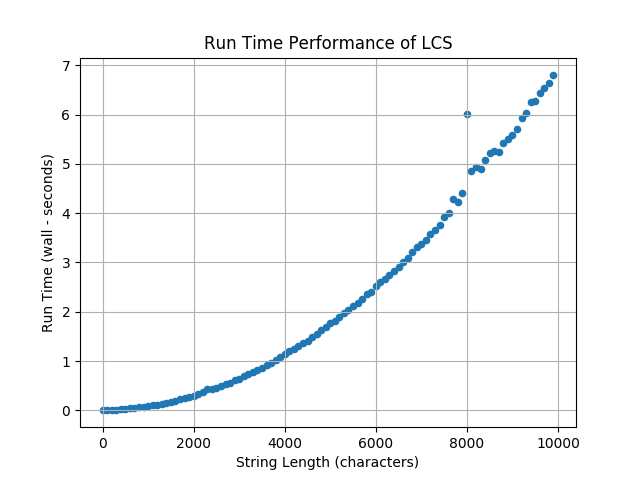
\includegraphics[width=10cm]{img/runtime_performance.png}
\end{figure}

The Python script can be run using the instructions in section B of the appendix.

\newpage

\chapter{Parallelisation of the Problem}
Given the typically $O(n^2)$ behaviour of the longest common sub-sequence problem, one way of accelerating the computation time is to break the problem up into distinct subsections and approach it in parallel. The following sections describe the approach taken to paralleise the problem using the OpenMP and Open MPI C++ libraries.

\section{Parallelisation Strategy}

% How did I make use of OpenMP?
\subsection{Multi-Threading with OpenMP}
Due to the fact that multiple threads can be run in a single process and that OpenMP utilises threads for its multi-processing, I decided early on that in order to maximise the performance of the program that the OpenMP optimisations would take place inside each MPI process.

Utilising OpenMP effectively proved challenging and required a complete overhaul of the serial code for populating the table described in Section 1.2 and visualised in Figure \ref{fig:table}. Instead of populating the table iteratively by row and column, cells were populated on the anti-diagonal (see Figure \ref{fig:techniques}). Because each cell only relies on the cells to its left and top, this allows every cell the entire anti-diagonal to be calculated simultaneously. In theory, if the same number of OpenMP threads were allocated to length of the diagonal, each cell in that diagonal could be calculated independently (and in parallel.

\begin{figure}[h]
\label{fig:techniques}
\centering
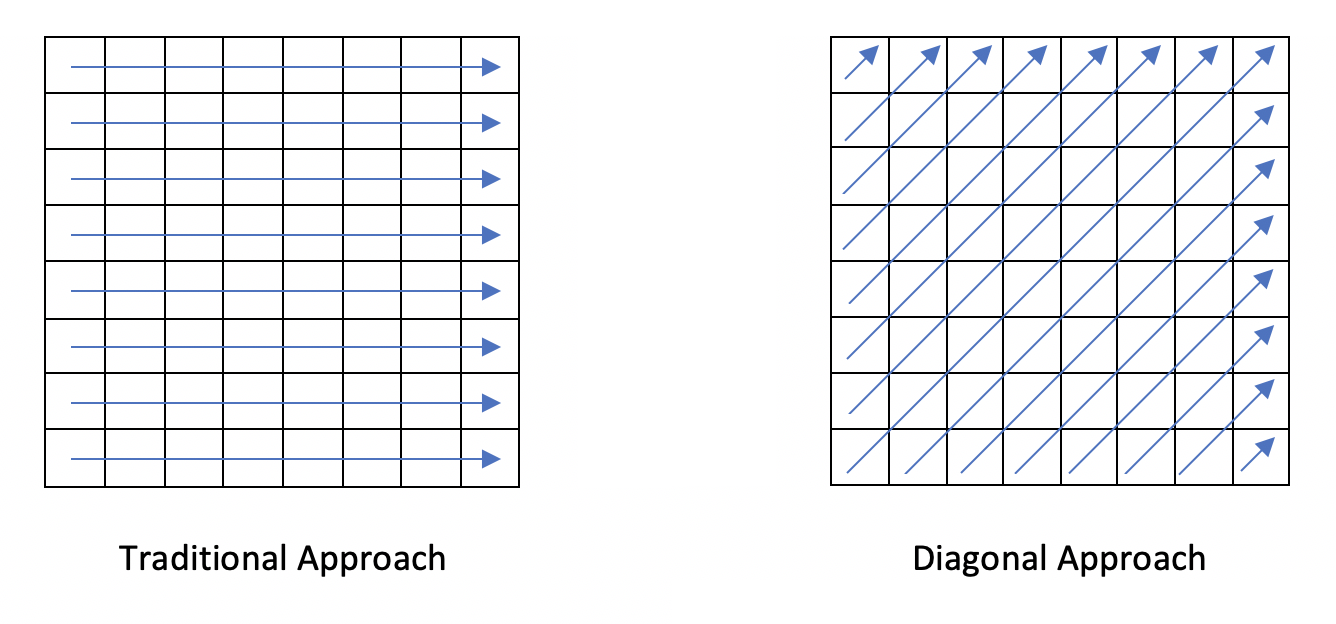
\includegraphics[width=12cm]{img/diagonal.png}
\caption{Population Techniques}
\end{figure}

This required the pre-computation of an order of execution more complicated than iterating over the length and height of the matrix. A C++ \lstinline{vector<vector<int>>} object was used to store the co-ordinates of each cell making up each "diagonal." These diagonals were then processed iteratively, with each constituent cell being processed in parallel using an OpenMPI \lstinline{parallel for} construct (see Listing 2.1).

\begin{lstlisting}[language=C++, caption=OpenMP Utilisation]
// The variable indices is vector<vector<int>> containing a list of diagonals
// which themselves contain (x, y) co-ordindate pairs.
for (int i = 0; i < (int) indices.size(); i++) {
    vector<vector<int>> diagonal = indices[i];
    #pragma omp parallel for shared(table, diagonal, a, b, top, left)
    for (int j = 0; j < (int) diagonal.size(); j++) {
        vector<int> cell = diagonal[j];
        int x = cell[0];
        int y = cell[1];
        int result = calculate_cell(table, x, y, a, b, top, left);
        table[y][x] = result;
    }
}
\end{lstlisting}

% How did I make use of MPI?
\subsection{Multi-Processing with OpenMPI}
Transforming the program so that it could make use of multiple processes was incredibly challenging. Splitting up the problem space into neat sub-sections was non-trivial, when accounting for the potential of irregularities around the "edges" of the parent matrix (i.e. "non-full" sections). The order in which the segments are processed is practically identical to that of the OpenMP calculations for each cell, but instead of individual cells being computed in parallel by threads, whole sections are computed in parallel by MPI processes (each internally using OpenMP for cell-level calculations). 

The number of processes provided to the program is fetched dynamically and determines the number of segments. One process is reserved for the parent or "master," with remainder being used as child, or "worker" processes. The number of segments in the anti-diagonal is matched to the number of processes so that at peak parallelism (when the most cells are able to be processed in parallel), the program can take full advantage.

In figure \ref{fig:segmentation} below, the program has been allocated five processes, four of which have been made worker processes. This has resulted in a diagonal size of four, and a total sub-section count of sixteen. Each set of sub-sections of the same colour represent "diagonals." Each sub-section in a diagonal can have its constituent cell values calculated in parallel with those of the other sub-sections in that diagonal. The white arrow indicates the direction that diagonals are processed. The red and violet sections (the first and last diagonals) are processed by the master process due to either being necessary for the first worker processes or requiring the output of all previous cells, respectively.

\begin{figure}[h]
\centering
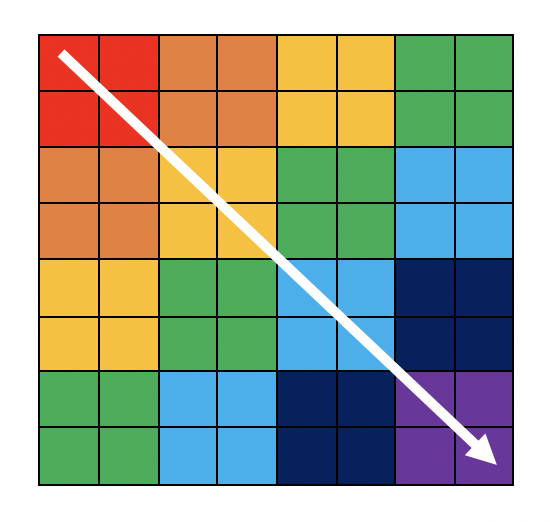
\includegraphics[width=5cm]{img/segments.png}
\caption{MPI Segmentation Technique}
\label{fig:segmentation}
\end{figure}

% How is information shared between threads and processes?
\subsection{Information Sharing}
\subsubsection{OpenMP}
Passing information to OpenMP was trivial due to the fact that each thread wrote to a discrete set of cells and read from cells that had already been populated (and would remain unchanged) in the calculation of the previous diagonal. In light of this, the master table was simply passed to each thread

\subsubsection{MPI}
Passing information was significantly more difficult between processes and required the use of the MPI message passing interface. For the computation of each sub-section additional data is required from the adjoining cells to the top and left. Figure \ref{fig:topleft} shows a single sub-segment (in orange) and the "top" (in blue) and "left" (in red) required to compute it. Each child, on inception, blocks and waits (using \lstinline{MPI_Recv()}) for three batches of information: the co-ordinates of the corners of the section being computed, the "top" data (converted into a one-dimentional \lstinline{int} array), and the "left" data (also converted), which are sent (using \lstinline{MPI_Send()}) by the master process. After computation, the contents of the subsection (in one-dimenional format) are sent back to the master process and are used to populate the master table.

\begin{figure}[h]
\centering
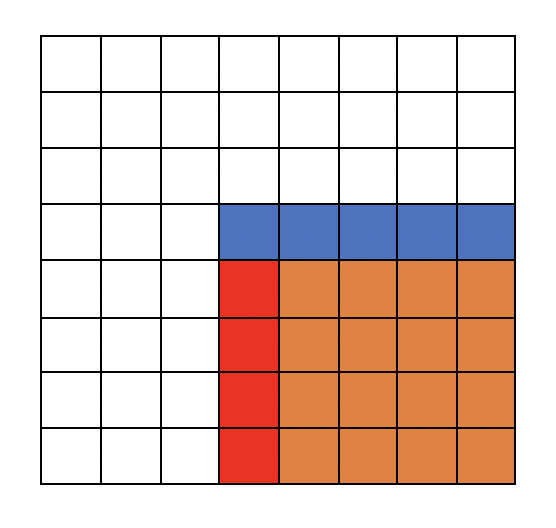
\includegraphics[width=5cm]{img/topleft.png}
\caption{Top (Blue) and Left (Red) Sections}
\label{fig:topleft}
\end{figure}

% Any optimisations investigated and/or challenges encountered will go here
\subsection{Challenges}
There were numerous false starts when devising a hybrid solution to the LCS problem. One particular example was a method devised by \cite{Li2017}. However, upon implementation it became apparent that the algorithm provided had several errors. It proved easier implementing, from scratch, the logic for handling both the OpenMP and MPI portions of the program.

Resource access was also a point of difficulty, particularly when trying to run tests with more than one or two processes (let alone multiple nodes) in the week leading up to the submission of milestone two.

Edge cases surrounding the behaviour of the program when assigned less than three processes were also encountered, overcome by reverting the application to utilising only OpenMP in these cases.

It also proved infeasible to parallelise the reconstruction of the longest common subsequence from the table (backtracking), as each step relied on the state acheived by the previous one. Many possibilities were considered but the nature of the problem procluded any obvious speedups from either OpenMP or MPI.

% A description of how you have verified the correctness of your parallel implementation. 
\section{Verification}
Due to the increased complexity of the code when deconstructing the problem to be performed over multiple threads and multiple processes it was essential to verify that the correctness of the program was maintained. The test suite from Section \ref{sec:correctness} was rerun under each of the following conditions:

\begin{itemize} 
    \item With a single MPI process.
    \item With three MPI processes (the lowest size that will trigger MPI multi-processing).
    \item With four MPI processes (typical usage).
    \item With sixteen MPI processes (high usage).
\end{itemize}

Each of these tests was run with an allocation of a single OpenMP thread (effectively serial), then again with with multiple threads.

\section{Scalability Test Plan}

\subsection{Strong Scaling}
Strong scaling measures the increase in performance for a fixed problem size. To test this form of scaling, two randomly generated strings of 100,000 each will be generated and run with the configurations in Table \ref{tab:strong}. These vary over two primary parameters: number of processes and number of threads. Due to the nature of the test clusters, when the number of processes exceeds the available number of CPU cores on a node, multiple nodes are used and the processes are split up evenly over multiple nodes.

\begin{table}[H]
\centering
\begin{tabular}{|l|l|l|l|}
\hline
\textbf{Nodes} & \textbf{\begin{tabular}[c]{@{}l@{}}Number of Tasks\\ (processes)\end{tabular}} & \textbf{Number of Tasks Per Node} & \textbf{\begin{tabular}[c]{@{}l@{}}CPUs Per Tasks\\ (threads)\end{tabular}} \\ \hline
1 & 1 & 1 & 1 \\ \hline
1 & 2 & 2 & 2 \\ \hline
1 & 4 & 4 & 4 \\ \hline
1 & 8 & 8 & 8 \\ \hline
1 & 16 & 16 & 8 \\ \hline
1 & 16 & 16 & 16 \\ \hline
1 & 16 & 16 & 32 \\ \hline
2 & 32 & 16 & 8 \\ \hline
2 & 32 & 16 & 16 \\ \hline
2 & 32 & 16 & 32 \\ \hline
4 & 64 & 16 & 32 \\ \hline
\end{tabular}
\caption{Strong Scaling Plan}
\label{tab:strong}
\end{table}

These runs will be run on UQ's \lstinline{goliath} cluster using \lstinline{slurm} (\lstinline{sbatch}) and a configuration shell script. An example script has been included in Appendix 3. Each run will be timed and compared to the serial solution and one another. The comparison with the serial solution will allow for the determination of how effective the solution is with respect to strong scaling or "speed up."

\subsection{Weak Scaling}
Weak scaling measures the effect of a program's parallelism as the size of the input changes. To test this type of scaling, I will run the same tests used for each of the following randomly generated string lengths:

\begin{table}[H]
\centering
\begin{tabular}{|l|}
\hline
\textbf{Input Length} \\ \hline
1 \\ \hline
10 \\ \hline
100 \\ \hline
1000 \\ \hline
10000 \\ \hline
100000 \\ \hline
\end{tabular}
\caption{Weak Scaling}
\label{tab:weak}
\end{table}

In order to offset any abnormalities caused by particular (randomly generated) input strings, each test will be run multiple times and averaged out. The \lstinline{testing.py} script used for the first milestone will be modified to support this behaviour.

% The idea here is that you could take this plan an start performing timing experiments. You should arrange testing so that if your test plan is curtailed, then you can still draw sensible conclusions from the results you do get.

\subsection{Test Plan Timeline}
In order to avoid the trouble I faced with respect to node availability, I expect to front-load a lot of the work for the final milestone. The table below outlines my timeline:

\begin{table}[H]
\centering
\begin{tabular}{|l|l|l|}
\hline
\textbf{Week} & \textbf{Activity} & \textbf{Rationale} \\ \hline
Midsemester Break & \begin{tabular}[c]{@{}l@{}}Development of testing.py \\ script for automating testing\end{tabular} & \begin{tabular}[c]{@{}l@{}}Automating the testing will save the \\ manual entry of parameters\end{tabular} \\ \hline
Week 11 & Strong Scaling & \begin{tabular}[c]{@{}l@{}}Strong scaling is the simple case and \\ can be tackled first\end{tabular} \\ \hline
Week 12 & Weak Scaling & \begin{tabular}[c]{@{}l@{}}This should be just the addition of extra \\ parameters (and iteration) to the strong scaling\end{tabular} \\ \hline
Week 13 & Buffer Time & \begin{tabular}[c]{@{}l@{}}I have left this space free in case testing\\  takes longer than expected, but would prefer\\  to avoid it as the clusters will be busy\end{tabular} \\ \hline
\end{tabular}
\caption{Timeline}
\label{tab:timeline}
\end{table}


% Remember that getafix is a shared facility so you are not guaranteed to get all the time you might like.
\clearpage

\newcommand\ddfrac[2]{\frac{\displaystyle #1}{\displaystyle #2}}

\chapter{Testing Parallelisation Efficiency}

\textbf{N.B: My code has changed significantly since Milestone 2, it has been committed to the MS3 directory of the provided SVN repository.}

\section{Test Framework}
To offset the tedious work of running the numerous tests outlined by the initial testing plan, the Python script developed for the basic testing carried out in Chapter 1 was extended to automate the process for both strong and weak testing. As such, the procedure for reproducing these results consists of only eleven commands, these can be found in Appendix \ref{app:framework}. 
This was accomplished by programmatically populating a \lstinline{slurm} template (found in Appendix \ref{app:template}) and submitting tasks using \lstinline{sbatch}. The script was also used to collate and summarise the output of the tests, producing both the results charts found below, and CSV reports of the findings. Single jobs can also be run by populating the template and running \lstinline{sbatch template.sh}.

\section{Deviations from Initial Test Plan}
Due to unforeseen limitations imposed by the available hardware on the \lstinline{goliath} and \lstinline{getafix} clusters where the tests were performed, both strong and weak scaling plans needed to be revised. Specifically, the fact that each node of the coursework partition contains only 64 cores proved a limiting factor. This was expected, but what was not expected was that the allocation of each thread to OpenMP would require the exclusive utilisation of a whole core.

\subsection{Strong Scaling}
% Table, Count, Technology Used
The strong scaling test plan was the most severely affected by the limitations described above. Previous plans to have configurations containing up to 32 threads were scrapped, and more configuration options were added due to the relative ease of assigning them programmaticaly. This primarily consisted of ensuring that each task/node configuration was tested using all compatible thread configurations. The final set of configurations can be found in Appendix \ref{app:actual-strong}. All tests were conducted on a problem size of 10,000 characters.

\subsection{Weak Scaling}
Due to a fundamental misunderstanding about how tests for weak scaling were to be performed, the test input sizes needed to be seriously curtailed as tests of 10,000 or 100,000 characters (per processing unit) would not be feasible due to the time limits imposed by the course. Test results for an input length of 1 character were discarded as they consisted entirely of noise. The final input length options are included in the table below. Each test of each configuration was conducted twenty times for each input size (problem size/processing unit). 
% Table, Count, Size Choice Justification

\begin{table}[H]
\centering
\begin{tabular}{|l|}
\hline
\multicolumn{1}{|c|}{\textbf{\begin{tabular}[c]{@{}c@{}}Input Size\\ (per processing unit)\end{tabular}}} \\ \hline
10 \\ \hline
100 \\ \hline
1000 \\ \hline
\end{tabular}
\caption{Actual Weak Scaling Input Magnitudes}
\label{tab:real-weak}
\end{table}


\section{Test Results}
\subsection{Strong Scaling}

Strong scaling tests were conducted on both the \lstinline{goliath} and \lstinline{getafix} clusters . A summary of mean results across the 20 samples collected for each configuration is included in Appendix \ref{app:strong-res}. Figure \ref{fig:strong-results} below shows the aggregated performance of the program on a fixed problem size of 10,000 characters, with varying combinations of MPI processes and OpenMP threads.

\begin{figure}[H]
\centering
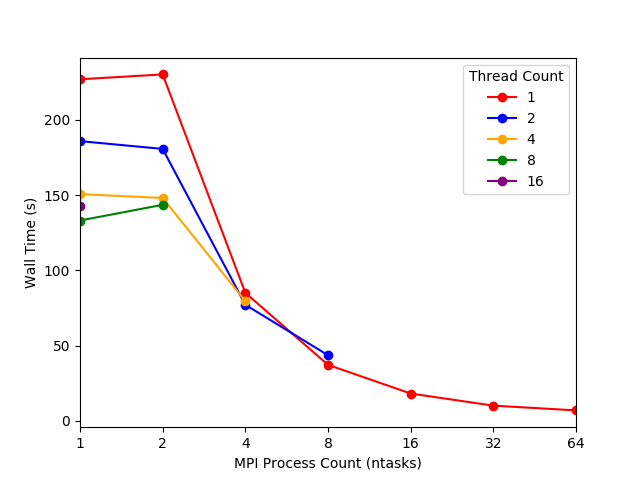
\includegraphics[width=10cm]{img/strong.png}
\caption{Strong Scaling Results}
\label{fig:strong-results}
\end{figure}

\subsubsection{Multi-threading Performance}
As can be seen in Figure \ref{fig:strong-results}, the addition of OpenMP threads has a distinct impact on overall run-time, particularly for configurations consisting of few MPI processes. However, the effect of additional threads has a diminishing rate of return, and can even be detrimental. This can be seen in the one-task, 16-thread configuration that has demonstrably worse performance than the one-task, eight-thread configuration even when averaged over 20 samples. The positive impact also (at $\geq$ 8 threads) diminishes quite rapidly; for example, the first additional thread reduces compute time by ~18\%, but it takes an additional two processes to achieve an additional performance impact of the same magnitude. More threads may have a significantly more beneficial impact on larger problem sizes, where the diagonal length of sub-sections far outstrips the number of threads available.

\subsubsection{Multi-processing Performance}
The addition of processes also had a clearly positive effect, far more impactful than that of threads. There is one notable exception, at the configuration involving two-task, one thread, which performed worse than with one-task. This makes sense in the context of the segmentation heuristic responsible for allocating work to child processes. Due to the complex nature of splitting the problem, configurations with two processes will short-circuit to using a single processor. Given the overhead of setting up a process and not using it, the difference in performance at $ntasks=2$ is to be expected. This problem is discussed in greater detail in section 3.5.3, below.

\subsection{Weak Scaling}

A summary of mean results across the 20 samples collected for each configuration of weak testing is included in Appendix \ref{app:weak-res}. Figure \ref{fig:weak-results} below plots the weak scaling results for the three different problem sizes (per unit). 

\begin{figure}[H]
\centering
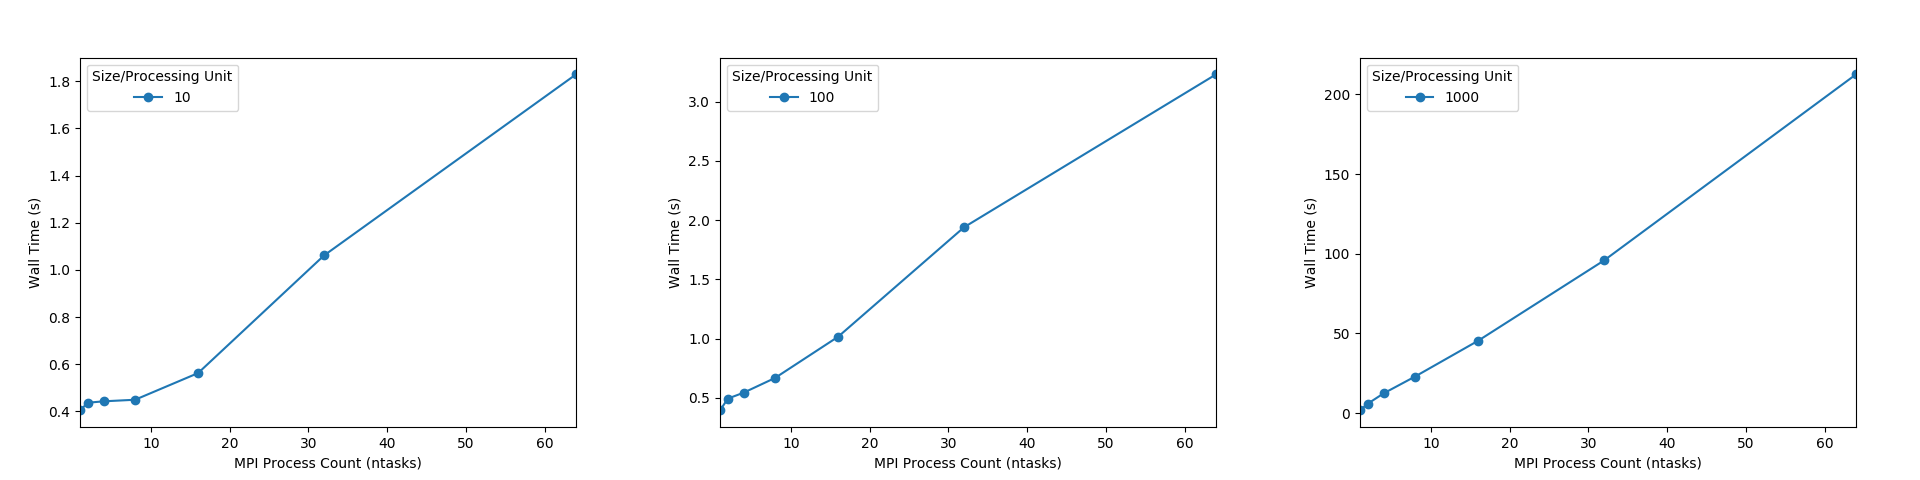
\includegraphics[width=18cm]{img/weak.png}
\caption{Weak Scaling Results}
\label{fig:weak-results}
\end{figure}

All three problem magnitudes appear to be growing extremely linearly with increased processing units and respective problem size, excepting a small amount of noise in the $n=10$ test results. This is deceptive, as we shall see in the efficiency analysis, because the absolute extent of the gradient is hidden by the axes' limits being set relative to the data points.

\section{Scaling Efficiency}
\subsection{Strong Scaling Efficiency}
Despite the strong apparent showing of the results in the previous section, examining the results in terms of "speed-up" relative to a serial solution, showed several surprising results. The following formula was used to calculate the actual speedup:
$$\frac{runtime_{serial}}{runtime_{parallel}}$$
This was compared to the theoretical maximum speedup as proposed by Amdahl \cite{Amdahl}, calculated with the following formula:
$$\frac{1}{\frac{f(N)}{p} + (1 - f(N))}$$
Where $N$ is the problem size, $p$ is the number of processing units and $f(N)$ is the proportion of the program's run-time that can be parallelised. Both threads and processes, given their requirement for a single core per unit, were treated as coequal processing units in the graph below. Due to the overwhelming proportion of time in the parallelisable section, this figure was set at 0.95 (i.e. 95\% of time was spent in parallelisable sections).

\begin{figure}[H]
\centering
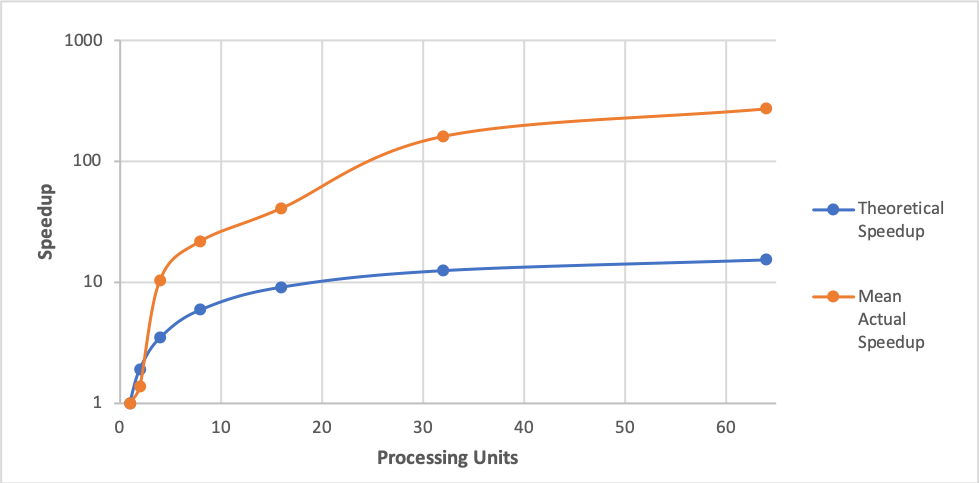
\includegraphics[width=10cm]{img/strong-scaling.png}
\caption{Strong Scaling Efficiency}
\label{fig:strong-efficiency}
\end{figure}

The first thing that stands out is that the actual speedup almost immediately overshoots the theoretical maximum by a non-trivial amount (note the logarithmic scale of the vertical axis). While this should not theoretically be possible (and had to be verified to ensure it was not a mistake) there are numerous possible explanations for this, the most likely being that the serial solution has been made artificially slow by the modification of the code to allow for the possibility of parallelisation. Other possible reasons could include environmental factors, though this is less likely due to the fact that twenty iterations were conducted and the mean taken.

\subsection{Weak Scaling Efficiency}

Weak scaling efficiency was calculated using the same formula as strong scaling, with a correction for the increasing problem size:
$$\frac{runtime_{pserial}}{runtime_{parallel} / processing\, units}$$
The theoretical maximum was calculated in accordance with the rule proposed by Gustafson \cite{Gustafson}:
$$p + (1 - p) \cdot T_{serial}$$
Where $T_{serial}$ is the proportion of time spent on serial (or non-parallelisable) sections of code.

\begin{figure}[H]
\centering
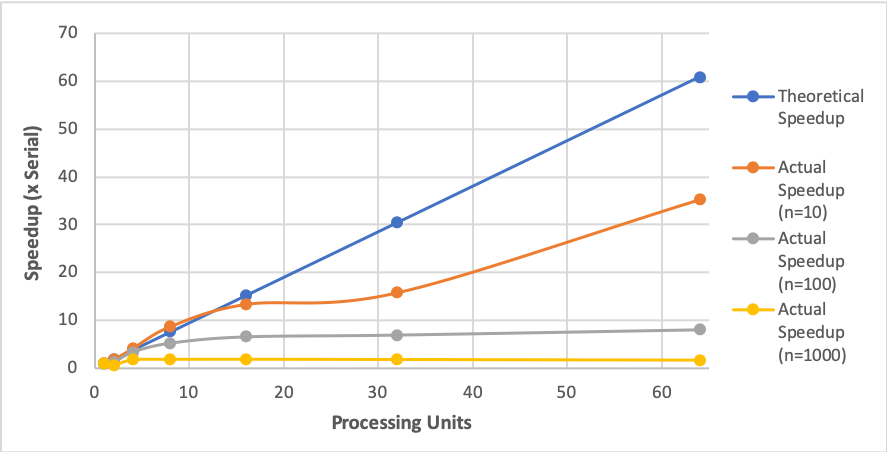
\includegraphics[width=10cm]{img/weak-scaling.png}
\caption{Weak Scaling Efficiency}
\label{fig:weak-efficiency}
\end{figure}

These figures are far more inline with expected behaviour, though below eight processing units the speedup still exceeded the theoretical maximum. Again, this could be due to noise given the small problem size, but the excessive sensitivity to the serial time is more likely to blame.

The behaviour of the tests at the $n=1000$ level was somewhat unexpected, as the larger problem size should have offset a lot of the communication and setup overhead, but on further inspection it became apparent that the communication load grows linearly with the problem size. However, this does not explain why the performance at this level is so much worse than linear. This could suggest a severe overestimation of the parallelisable proportion of the code, but such a hypothesis would not be consistent with the results of the strong scaling tests.

\section{Findings}
\subsection{Impediments}
There were numerous instances in which errors in programming or test design led to less than satisfactory outcomes during the course of development and testing of the parallel LCS solution. Several of the most impactful of these have been summarised below: 
\begin{itemize}
    \item Memory Allocation: initial phases of testing were conducted under simple conditions, and total input size never exceeded a character length of 10,000 (resulting in a table size of 100 million elements). However, on proceeding to larger input sizes, memory allocation for the table contained in the master process began to fail. In order to optimise on memory usage, the entire codebase was translated from using C++ \lstinline{std::vector} objects to using raw integer arrays to store the master and sub-section tables. This proved insufficient, as it later emerged that the master table was being constructed (duplicated) in every process, despite being unused in worker processes. Removal of this bug allowed for normal operation until significantly larger problem sizes (\textgreater 2.5 billion element master tables) where the problem re-emerged. This was solved by requesting larger memory allocations in the \lstinline{slurm} shell scripts submitted to \lstinline{sbatch}.
    \item Resource Binding: another problem encountered due to my relative naivete with respect \lstinline{slurm} and programming for clusters was not realising that, by default, OpenMP threads allocated to the job will be bound to a single core. This was overcome by passing the \lstinline{--bind-to none} flag to \lstinline{mpirun}. The incredible impact of this change on performance can be seen in Figure \ref{fig:resource-binding}, though these results were confounded by a change in cluster from \lstinline{goliath} to \lstinline{getafix}. Notice in particular the order of magnitude change in run time. This reduced run time also impacts the uniformity of the results, despite both test runs containing the same number of samples.
    \begin{figure}[H]
    \centering
    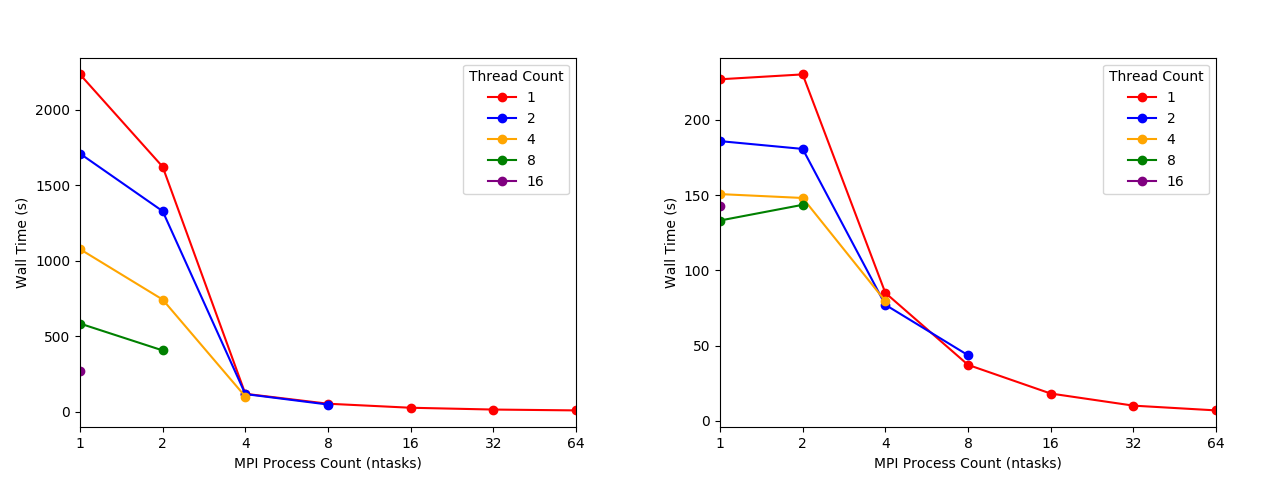
\includegraphics[width=18cm]{img/resource-binding.png}
    \caption{Pre-Resource Binding (left, goliath) and Post Resource Binding (right, getafix)}
    \label{fig:resource-binding}
    \end{figure}
    \item Level of Threading Support: my initial plans for parallelising the distribution of work to worker processes involved using OpenMP to have each send and receipt completed by a separate thread, IO-heavy work being a perfect place to implement threading. Unfortunately this implementation would have required a level of threading support (\lstinline{MPI_THREAD_MULTIPLE}) not supported on either \lstinline{goliath} or \lstinline{getafix} (both of which only support \lstinline{MPI_THREAD_SERIALIZED}); the level being set at compile-time (both clusters being compiled). This would have allowed for OpenMP multi-threading in both the master and worker classes simultaneously. Though not implemented, alternative options for parallelising this section are discussed below.
\end{itemize}

\subsection{Strengths}

The primary strength of the approach taken is that it takes full advantage of the multi-processing capabilities of the clusters on which it was tested. By utilising the diagonal calculation methodology at both the thread and process level, the program was able to achieve speed-ups in excess of the theoretical maximum. Though this is likely due to poor serial performance, it does indicate that the parallelisation has been particularly successful.

\subsection{Weaknesses \& Possible Improvements}

There are numerous areas in which the program, as written, lacks sophistication and could stand to be improved. Three of the most serious issues have been detailed below.

\subsubsection{Problem Division}
By far the greatest weakness of the parallel algorithm as it stands is the relatively naive way in which the problem space is divided into sub-problems, and the way these sub-problems are allocated to worker processes.

The diagonal calculation algorithm utilised in the program is most efficient when sub-sections are perfectly square. This enables the most threads to simultaneously calculate cells. The present heuristic divides the total problem into $n \cdot n$ subsections (where $n$ is the number of processes), without considering the dimensions of the problem. A more advanced heuristic considering these factors, and the relative importance of prioritising the size optimality of the whole problem (where each sub-section is dealt with by processes) against that of the subsections (where each cell on a diagonal may be calculated by independent threads). Dynamic detection of the number of and threads (in addition to that of processes, which is already utilised) may assist in optimising performance in this area.

\subsubsection{Allocation}
In order to simplify the process of allocating and distributing process, the program short-circuits parallel operation for any less than three processors, due to difficulties imposed by the previously mentioned segmentation heuristic. Optimally, the actual segmentation would remain unchanged, but each sub-section would be allocated to the sole worker process in order. The master process could also be utilised for more actual calculations, making use of the downtime between sending and receiving large sub-sections from worker processes.

\subsubsection{Distribution}
Due to numerous, significant, and time-consuming problems in implementing asynchronous behaviour, all MPI send and receive operations are conducted synchronously. It is strongly recommended that the sending of sub-section data to worker processes and the receipt of completed sub-sections be conducted in parallel. The nature of the algorithm would necessitate that all sub-sections on a diagonal be finished before the next begins. Hence, an \lstinline{MPI_Waitall} will be required between diagonals. There is no discernible benefit in asynchronously sending and receiving on the worker-process end, due to the linear nature of their operation.

\subsection{Further Scaling}
The range of testing configurations was severely limited by the resources allocated to the course, specifically the number of nodes available on the \lstinline{getafix} $cosc$ and \lstinline{goliath} $coursework$ partitions. Time was also a limiting factor as due to the shared nature of these resources.

In order to support truly massive input sizes, the program would need to be modified to offset limitations imposed by a lack of available hardware. 

Memory proved to be the most pressing resource constraint in the small-scale testing conducted for this report, and there is no reason to expect this would not be the case for even larger input sizes. The sheer size of the master table (already in the billions of elements for conducted tests) will eventually result in a lack of sufficient RAM to store the table. This could be offset by keeping only those values necessary for computation in memory and storing already computed values on disk. Entire sections could be saved to files and reloaded on demand. This would introduce additional IO overhead, but may be unavoidable and would certainly be offset by sufficient processing gains. This would also have the advantage of providing progress "checkpoints" that may allow for the resumption of processing in the event of interruption.

Processing power will also (eventually) hit physical limitations. It may be worth modifying the division of the problem such that the number of segments on the major anti-diagonal outnumbers the process count, such that each each segment is computable in a reasonable amount of time with the (potentially) limited resources of each node. This would introduce additional logical complexity in the distribution and receipt of segments, but may produce additional performance gains in the event of a cluster consisting of a high number of low resource nodes.

% Section Header

\newpage

\bibliography{bibliography} 
\bibliographystyle{ieeetr}

\newpage

\titlespacing\chapter{0pt}{0pt}{0pt}
\titleformat{\chapter}[display]{\bfseries}{\huge\appendixname~\thechapter}{2ex}{\LARGE}

\begin{appendices}

\chapter{Running the Program (Deprecated)}

\begin{lstlisting}[language=bash, caption=Usage Instructions, captionpos=b]
svn co https://source.eait.uq.edu.au/svn/cosc3500-s4261833/trunk/MS1
cd MS1
make
./bin/lcs test_input.txt test_output.txt
\end{lstlisting}

\chapter{Running the Performance Tests (Deprecated)}
\begin{lstlisting}[language=bash, caption=Usage Instructions, captionpos=b]
svn co https://source.eait.uq.edu.au/svn/cosc3500-s4261833/trunk/MS1
cd MS1
make
python3 -m venv venv
source venv/bin/activate
pip install -r requirements.txt
python -m testing <num_tests> <max_length>
\end{lstlisting}

\chapter{Slurm Script}
\begin{lstlisting}[language=bash, caption=Slurm Script (go.sh), captionpos=b]
#!/bin/bash
#SBATCH −−partition=coursework
#SBATCH −−job−name=:sad_parrot:
#SBATCH −−nodes=1
#SBATCH −−ntasks=4
#SBATCH −−ntasks−per−node=4
#SBATCH −−cpus−per−task=4

export OMP_NUM_THREADS=4
export SLURM_TASKS_PER_NODE=4
export SLURM_NPROCS=4

DATE=$(date +"%Y%m%d%H%M")
echo "time started "$DATE
echo "This is job ’$SLURM_JOB_NAME’ (id: $SLURM_JOB_ID) running on the following nodes:"
echo $SLURM_NODELIST
echo "running with OMP_NUM_THREADS= $OMP_NUM_THREADS "
echo "running with SLURM_TASKS_PER_NODE= $SLURM_TASKS_PER_NODE "
echo "running with SLURM_NPROCS= $SLURM_NPROCS "
echo "Now we start the show:"
export TIMEFORMAT="%E sec"

module load mpi/openmpi-x86_64
time mpirun -n ${SLURM_NPROCS} ./bin/lcs-hybrid test_input.txt test_output.txt

DATE=$(date +"%Y%m%d%H%M")
echo "time finished "$DATE
# echo "we just ran with the following SLURM environment variables" # env | grep SLURM
\end{lstlisting}


\chapter{Testing Framework Operation}
\label{app:framework}
\begin{lstlisting}[language=bash, caption=Testing Framework Operation, captionpos=b]
svn co https://source.eait.uq.edu.au/svn/cosc3500-s4261833/trunk/MS3

make

python3 -m venv venv
source venv/bin/activate
pip install -r requirements.txt

python -m testing run strong 10000 20
# Wait for the resulting slurm jobs to finish
mv ./tests ./tests-strong
python -m testing report strong ./tests-strong

python -m testing run weak 20
# Wait for the resulting slurm jobs to finish
mv ./tests ./tests-weak
python -m testing report weak ./tests-weak
\end{lstlisting}


\chapter{Slurm Template}
\label{app:template}
\begin{lstlisting}[language=bash, caption=Slurm Template (template.sh), captionpos=b]
#!/bin/bash
#SBATCH --partition=coursework
#SBATCH --job-name={{name}}
#SBATCH --nodes={{nnodes}}
#SBATCH --ntasks={{ntasks}}
#SBATCH --ntasks-per-node={{ntasks_per_node}}
#SBATCH --cpus-per-task={{cpus_per_task}}
#SBATCH --time=1:00:00

export OMP_NUM_THREADS=${SLURM_CPUS_PER_TASK}
export TIMEFORMAT="%E sec"

echo "{{name}} - {{input}}"

module load mpi/openmpi-x86_64
time mpirun -n ${SLURM_NPROCS} {{binary}} {{input}} {{output}}

DATE=$(date +"%Y%m%d%H%M")
echo "time finished "$DATE
\end{lstlisting}

\chapter{Actual Strong Testing Configuration}
\label{app:actual-strong}

\begin{table}[H]
\centering
\begin{tabular}{|l|l|l|l|}
\hline
\multicolumn{1}{|c|}{\textbf{Nodes}} & \multicolumn{1}{c|}{\textbf{Tasks}} & \multicolumn{1}{c|}{\textbf{Tasks/Node}} & \multicolumn{1}{c|}{\textbf{CPUs/Task}} \\ \hline
1 & 1 & 1 & 1 \\ \hline
1 & 1 & 1 & 2 \\ \hline
1 & 1 & 1 & 4 \\ \hline
1 & 1 & 1 & 8 \\ \hline
1 & 1 & 1 & 16 \\ \hline
1 & 2 & 2 & 1 \\ \hline
1 & 2 & 2 & 2 \\ \hline
1 & 2 & 2 & 4 \\ \hline
1 & 2 & 2 & 8 \\ \hline
1 & 4 & 4 & 1 \\ \hline
1 & 4 & 4 & 2 \\ \hline
1 & 4 & 4 & 4 \\ \hline
1 & 8 & 8 & 1 \\ \hline
1 & 8 & 8 & 2 \\ \hline
1 & 16 & 16 & 1 \\ \hline
2 & 2 & 1 & 1 \\ \hline
2 & 2 & 1 & 2 \\ \hline
2 & 2 & 1 & 4 \\ \hline
2 & 2 & 1 & 8 \\ \hline
2 & 4 & 2 & 1 \\ \hline
2 & 4 & 2 & 2 \\ \hline
2 & 4 & 2 & 4 \\ \hline
2 & 8 & 4 & 1 \\ \hline
2 & 8 & 4 & 2 \\ \hline
2 & 16 & 8 & 1 \\ \hline
2 & 32 & 16 & 1 \\ \hline
4 & 4 & 1 & 1 \\ \hline
4 & 4 & 1 & 2 \\ \hline
4 & 4 & 1 & 4 \\ \hline
4 & 8 & 2 & 1 \\ \hline
4 & 8 & 2 & 2 \\ \hline
4 & 16 & 4 & 1 \\ \hline
4 & 32 & 8 & 1 \\ \hline
4 & 64 & 16 & 1 \\ \hline
\end{tabular}
\caption{Strong Scaling Test Configuration}
\label{tab:strong-config}
\end{table}

\chapter{Full Strong Scaling Results}
\label{app:strong-res}

\begin{table}[H]
\centering
\begin{tabular}{|l|l|l|l|l|l|l|l|l|l|}
\hline
\multicolumn{1}{|c|}{\textbf{Nodes}} & \multicolumn{1}{c|}{\textbf{Tasks}} & \multicolumn{1}{c|}{\textbf{\begin{tabular}[c]{@{}c@{}}Tasks/\\ Node\end{tabular}}} & \multicolumn{1}{c|}{\textbf{\begin{tabular}[c]{@{}c@{}}CPUs/\\ Task\end{tabular}}} & \multicolumn{1}{c|}{\textbf{\begin{tabular}[c]{@{}c@{}}Problem\\ Size\end{tabular}}} & \multicolumn{1}{c|}{\textbf{\begin{tabular}[c]{@{}c@{}}Problem\\ Size/\\ Task\end{tabular}}} & \multicolumn{1}{c|}{\textbf{\begin{tabular}[c]{@{}c@{}}Run\\ Time\end{tabular}}} & \multicolumn{1}{c|}{\textbf{\begin{tabular}[c]{@{}c@{}}Processing\\ Units\end{tabular}}} & \multicolumn{1}{c|}{\textbf{\begin{tabular}[c]{@{}c@{}}Theoretical\\ Speedup\end{tabular}}} & \multicolumn{1}{c|}{\textbf{\begin{tabular}[c]{@{}c@{}}Actual\\ Speedup\end{tabular}}} \\ \hline
1 & 1 & 1 & 1 & 10000 & 10000 & 226.8824 & 1 & 1.00 & 1.00 \\ \hline
1 & 1 & 1 & 2 & 10000 & 10000 & 185.8092 & 2 & 1.90 & 1.22 \\ \hline
1 & 1 & 1 & 4 & 10000 & 10000 & 150.6327 & 4 & 3.48 & 1.51 \\ \hline
1 & 1 & 1 & 8 & 10000 & 10000 & 133.09 & 8 & 5.93 & 1.70 \\ \hline
1 & 1 & 1 & 16 & 10000 & 10000 & 142.4498 & 16 & 9.14 & 1.59 \\ \hline
1 & 2 & 2 & 1 & 10000 & 5000 & 228.7812 & 2 & 1.90 & 0.99 \\ \hline
1 & 2 & 2 & 2 & 10000 & 5000 & 178.9482 & 4 & 3.48 & 1.27 \\ \hline
1 & 2 & 2 & 4 & 10000 & 5000 & 148.2034 & 8 & 5.93 & 1.53 \\ \hline
1 & 2 & 2 & 8 & 10000 & 5000 & 146.5848 & 16 & 9.14 & 1.55 \\ \hline
1 & 4 & 4 & 1 & 10000 & 2500 & 84.7677 & 4 & 3.48 & 2.68 \\ \hline
1 & 4 & 4 & 2 & 10000 & 2500 & 77.944 & 8 & 5.93 & 2.91 \\ \hline
1 & 4 & 4 & 4 & 10000 & 2500 & 82.579 & 16 & 9.14 & 2.75 \\ \hline
1 & 8 & 8 & 1 & 10000 & 1250 & 36.5175 & 8 & 5.93 & 6.21 \\ \hline
1 & 8 & 8 & 2 & 10000 & 1250 & 60.5753 & 16 & 9.14 & 3.75 \\ \hline
1 & 16 & 16 & 1 & 10000 & 625 & 18.1023 & 16 & 9.14 & 12.53 \\ \hline
2 & 2 & 1 & 1 & 10000 & 5000 & 231.4666 & 2 & 1.90 & 0.98 \\ \hline
2 & 2 & 1 & 2 & 10000 & 5000 & 182.3175 & 4 & 3.48 & 1.24 \\ \hline
2 & 2 & 1 & 4 & 10000 & 5000 & 147.9168 & 8 & 5.93 & 1.53 \\ \hline
2 & 2 & 1 & 8 & 10000 & 5000 & 140.4557 & 16 & 9.14 & 1.62 \\ \hline
2 & 4 & 2 & 1 & 10000 & 2500 & 85.2426 & 4 & 3.48 & 2.66 \\ \hline
2 & 4 & 2 & 2 & 10000 & 2500 & 78.4404 & 8 & 5.93 & 2.89 \\ \hline
2 & 4 & 2 & 4 & 10000 & 2500 & 83.6625 & 16 & 9.14 & 2.71 \\ \hline
2 & 8 & 4 & 1 & 10000 & 1250 & 37.9601 & 8 & 5.93 & 5.98 \\ \hline
2 & 8 & 4 & 2 & 10000 & 1250 & 35.2048 & 16 & 9.14 & 6.44 \\ \hline
2 & 16 & 8 & 1 & 10000 & 625 & 18.3757 & 16 & 9.14 & 12.35 \\ \hline
2 & 32 & 16 & 1 & 10000 & 312 & 10.2094 & 32 & 12.55 & 22.22 \\ \hline
4 & 4 & 1 & 1 & 10000 & 2500 & 85.1312 & 4 & 3.48 & 2.67 \\ \hline
4 & 4 & 1 & 2 & 10000 & 2500 & 74.9924 & 8 & 5.93 & 3.03 \\ \hline
4 & 4 & 1 & 4 & 10000 & 2500 & 72.5175 & 16 & 9.14 & 3.13 \\ \hline
4 & 8 & 2 & 1 & 10000 & 1250 & 37.2422 & 8 & 5.93 & 6.09 \\ \hline
4 & 8 & 2 & 2 & 10000 & 1250 & 35.1404 & 16 & 9.14 & 6.46 \\ \hline
4 & 16 & 4 & 1 & 10000 & 625 & 18.0858 & 16 & 9.14 & 12.54 \\ \hline
4 & 32 & 8 & 1 & 10000 & 312 & 10.0879 & 32 & 12.55 & 22.49 \\ \hline
4 & 64 & 16 & 1 & 10000 & 156 & 6.9848 & 64 & 15.42 & 32.48 \\ \hline
\end{tabular}
\caption{Full Strong Scaling Results (getafix, n=20)}
\label{tab:strong-results}
\end{table}

\chapter{Weak Scaling Results}
\label{app:weak-res}

\begin{table}[H]
\centering
\begin{tabular}{|l|l|l|l|l|l|l|l|l|l|}
\hline
\multicolumn{1}{|c|}{\textbf{Nodes}} & \multicolumn{1}{c|}{\textbf{Tasks}} & \multicolumn{1}{c|}{\textbf{\begin{tabular}[c]{@{}c@{}}Tasks/\\ Node\end{tabular}}} & \multicolumn{1}{c|}{\textbf{\begin{tabular}[c]{@{}c@{}}CPUs/\\ Task\end{tabular}}} & \multicolumn{1}{c|}{\textbf{\begin{tabular}[c]{@{}c@{}}Problem\\ Size\end{tabular}}} & \multicolumn{1}{c|}{\textbf{\begin{tabular}[c]{@{}c@{}}Problem\\ Size/Task\end{tabular}}} & \multicolumn{1}{c|}{\textbf{\begin{tabular}[c]{@{}c@{}}Run\\ Time\end{tabular}}} & \multicolumn{1}{c|}{\textbf{\begin{tabular}[c]{@{}c@{}}Processing\\ Units\end{tabular}}} & \multicolumn{1}{c|}{\textbf{\begin{tabular}[c]{@{}c@{}}Theoretical\\ Speedup\end{tabular}}} & \multicolumn{1}{c|}{\textbf{\begin{tabular}[c]{@{}c@{}}Actual\\ Speedup\end{tabular}}} \\ \hline
1 & 1 & 1 & 1 & 10 & 10 & 0.434 & 1 & 1 & 1.00 \\ \hline
1 & 2 & 2 & 1 & 20 & 10 & 0.465 & 2 & 1.95 & 1.86 \\ \hline
1 & 4 & 4 & 1 & 40 & 10 & 0.414 & 4 & 3.85 & 4.19 \\ \hline
1 & 8 & 8 & 1 & 80 & 10 & 0.395 & 8 & 7.65 & 8.78 \\ \hline
1 & 16 & 16 & 1 & 160 & 10 & 0.518 & 16 & 15.25 & 13.40 \\ \hline
2 & 32 & 16 & 1 & 320 & 10 & 0.877 & 32 & 30.45 & 15.83 \\ \hline
4 & 64 & 16 & 1 & 640 & 10 & 0.787 & 64 & 60.85 & 35.25 \\ \hline
1 & 1 & 1 & 1 & 100 & 100 & 0.462 & 1 & 1 & 1.00 \\ \hline
1 & 2 & 2 & 1 & 200 & 100 & 0.749 & 2 & 1.95 & 1.23 \\ \hline
1 & 4 & 4 & 1 & 400 & 100 & 0.551 & 4 & 3.85 & 3.36 \\ \hline
1 & 8 & 8 & 1 & 800 & 100 & 0.700 & 8 & 7.65 & 5.28 \\ \hline
1 & 16 & 16 & 1 & 1600 & 100 & 1.119 & 16 & 15.25 & 6.61 \\ \hline
2 & 32 & 16 & 1 & 3200 & 100 & 2.114 & 32 & 30.45 & 6.99 \\ \hline
4 & 64 & 16 & 1 & 6400 & 100 & 3.644 & 64 & 60.85 & 8.11 \\ \hline
1 & 1 & 1 & 1 & 1000 & 1000 & 8.036 & 1 & 1 & 1.00 \\ \hline
1 & 2 & 2 & 1 & 2000 & 1000 & 24.439 & 2 & 1.95 & 0.66 \\ \hline
1 & 4 & 4 & 1 & 4000 & 1000 & 17.651 & 4 & 3.85 & 1.82 \\ \hline
1 & 8 & 8 & 1 & 8000 & 1000 & 33.397 & 8 & 7.65 & 1.92 \\ \hline
1 & 16 & 16 & 1 & 16000 & 1000 & 66.100 & 16 & 15.25 & 1.95 \\ \hline
2 & 32 & 16 & 1 & 32000 & 1000 & 136.411 & 32 & 30.45 & 1.89 \\ \hline
4 & 64 & 16 & 1 & 64000 & 1000 & 292.969 & 64 & 60.85 & 1.76 \\ \hline
\end{tabular}
\caption{Full Weak Scaling Results}
\label{tab:weak-results}
\end{table}

\end{appendices}

\end{document}
}